% Generated by models/social_gan/handoff.py from audited results.
\providecommand{\SocialGanInsight}[1]{\csname social-gan:#1\endcsname}
\expandafter\def\csname social-gan:OneSampleADE\endcsname{0.835}
\expandafter\def\csname social-gan:BudgetReduction\endcsname{61}
\expandafter\def\csname social-gan:MaxSeedSD\endcsname{0.027}
\expandafter\def\csname social-gan:NoiseMaxFoldDelta\endcsname{+0.556}
\expandafter\def\csname social-gan:NoiseMinFoldDelta\endcsname{+0.342}
\expandafter\def\csname social-gan:UnivRuntime\endcsname{17.6}
\expandafter\def\csname social-gan:CleanSpeedViolationPct\endcsname{5.7}
\expandafter\def\csname social-gan:CleanCloseApproachPct\endcsname{87.6}
\expandafter\def\csname social-gan:FixedCleanMinADE\endcsname{1.015}
\expandafter\def\csname social-gan:FixedNoiseMinADE\endcsname{0.565}
\expandafter\def\csname social-gan:FailureMinADE\endcsname{4.692}
\expandafter\def\csname social-gan:FailureCoTargets\endcsname{15}
\expandafter\def\csname social-gan:FailureHeading\endcsname{174}
\expandafter\def\csname social-gan:ETHMinADE\endcsname{0.633}
\expandafter\def\csname social-gan:ETHMinFDE\endcsname{1.233}
\expandafter\def\csname social-gan:ETHMeanADE\endcsname{1.151}
\expandafter\def\csname social-gan:ETHMeanFDE\endcsname{2.415}
\expandafter\def\csname social-gan:ETHEnergy\endcsname{0.982}
\expandafter\def\csname social-gan:ETHDiversity\endcsname{0.805}
\expandafter\def\csname social-gan:HotelMinADE\endcsname{0.207}
\expandafter\def\csname social-gan:HotelMinFDE\endcsname{0.380}
\expandafter\def\csname social-gan:HotelMeanADE\endcsname{0.790}
\expandafter\def\csname social-gan:HotelMeanFDE\endcsname{1.658}
\expandafter\def\csname social-gan:HotelEnergy\endcsname{0.431}
\expandafter\def\csname social-gan:HotelDiversity\endcsname{1.033}
\expandafter\def\csname social-gan:UnivMinADE\endcsname{0.333}
\expandafter\def\csname social-gan:UnivMinFDE\endcsname{0.632}
\expandafter\def\csname social-gan:UnivMeanADE\endcsname{0.783}
\expandafter\def\csname social-gan:UnivMeanFDE\endcsname{1.641}
\expandafter\def\csname social-gan:UnivEnergy\endcsname{0.559}
\expandafter\def\csname social-gan:UnivDiversity\endcsname{0.753}
\expandafter\def\csname social-gan:Zara1MinADE\endcsname{0.233}
\expandafter\def\csname social-gan:Zara1MinFDE\endcsname{0.408}
\expandafter\def\csname social-gan:Zara1MeanADE\endcsname{0.766}
\expandafter\def\csname social-gan:Zara1MeanFDE\endcsname{1.567}
\expandafter\def\csname social-gan:Zara1Energy\endcsname{0.438}
\expandafter\def\csname social-gan:Zara1Diversity\endcsname{0.952}
\expandafter\def\csname social-gan:Zara2MinADE\endcsname{0.204}
\expandafter\def\csname social-gan:Zara2MinFDE\endcsname{0.362}
\expandafter\def\csname social-gan:Zara2MeanADE\endcsname{0.706}
\expandafter\def\csname social-gan:Zara2MeanFDE\endcsname{1.460}
\expandafter\def\csname social-gan:Zara2Energy\endcsname{0.383}
\expandafter\def\csname social-gan:Zara2Diversity\endcsname{0.917}


\begin{frame}{Social-GAN pools observed neighbors before decoding}
\small
\begin{columns}[T,onlytextwidth]
\column{.48\textwidth}
\textcolor{Teal}{\bfseries Observed context}\par\smallskip
One LSTM encodes the target and each visible neighbor. A learned max pool
summarizes neighbor motion and relative position at the anchor.
\column{.46\textwidth}
\textcolor{Teal}{\bfseries Sampled futures}\par\smallskip
A Gaussian draw initializes the decoder with that context. The decoder
adds a learned correction to constant velocity over 12 steps.
\end{columns}
\bigskip
\begin{block}{Two training signals}
An LSTM discriminator scores real and generated trajectories.
The variety loss updates the closest of 20 draws for each target.
\end{block}
\vfill
{\scriptsize\color{Muted}Cheung Alan Pak To\hfill Gupta et al., CVPR 2018}
\end{frame}

\begin{frame}{More draws improve the best match}
\small
\begin{columns}[T,onlytextwidth]
\column{.58\textwidth}
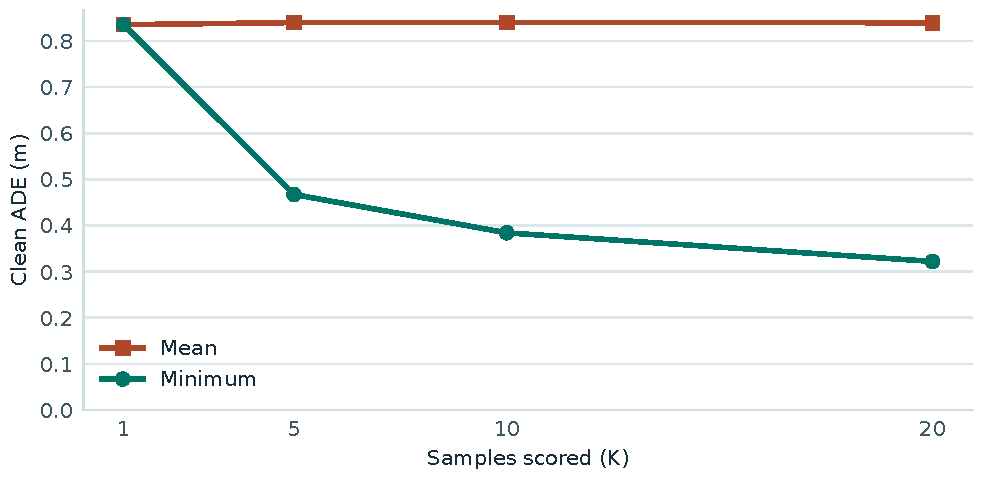
\includegraphics[width=\linewidth]{contributions/social_gan/assets/sampling.pdf}
\column{.38\textwidth}
\textcolor{Teal}{\bfseries Clean ADE at \(K=20\)}\par\smallskip
\ModelMetric{social_gan}{clean_0}{min_ade_mean}\,m minimum\par
\ModelMetric{social_gan}{clean_0}{mean_ade_mean}\,m mean\par
\medskip
The minimum uses the recorded future to pick a draw. The mean describes
the expected error of a uniformly chosen draw.\par
\medskip
0.20\,m input noise changed meanADE by
\ModelMeanADEChange{social_gan}{noise_020}\,m.
\end{columns}
\vfill
{\scriptsize\color{Muted}Cheung Alan Pak To\hfill Five holdouts, three seeds}
\end{frame}

\begin{frame}{Twenty samples can still miss a trajectory}
\centering
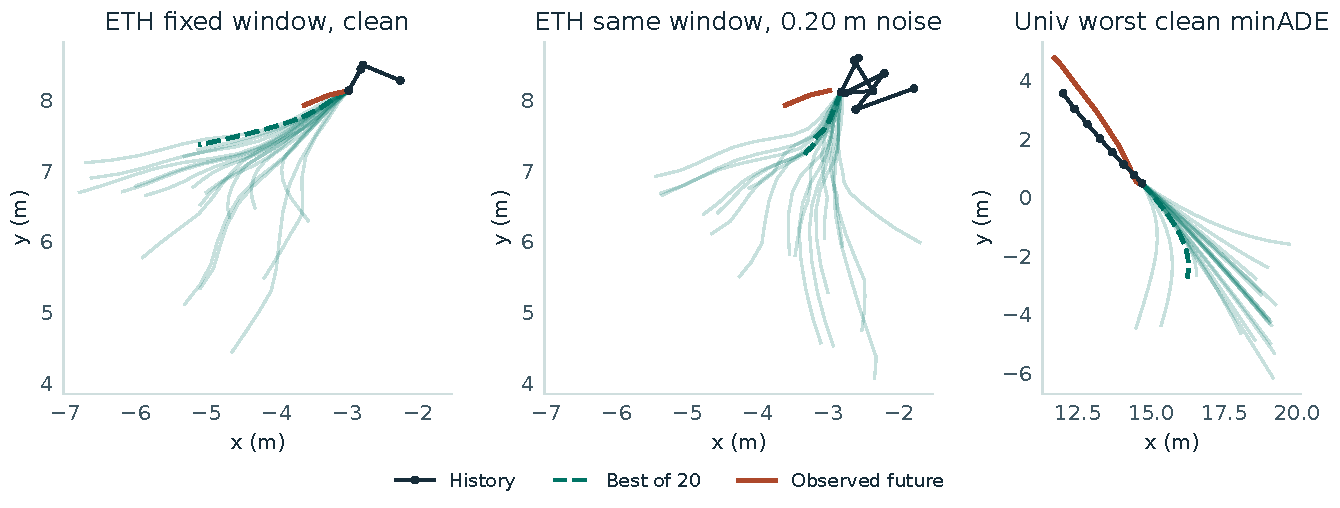
\includegraphics[width=.92\linewidth,height=4.65cm,keepaspectratio]{contributions/social_gan/assets/trajectory_examples.pdf}\par
\smallskip
{\small Same ETH window and draws on the left. Worst clean Univ window at seed 0 on the right.}\par
\vfill
\raggedright
{\scriptsize\color{Muted}Cheung Alan Pak To\hfill
\ModelRuntime{social_gan}{end_to_end_ms}\,ms per 128 targets on Apple M5 Pro CPU}
\end{frame}
